\documentclass[a3,2col]{ostposter}
%\documentclass[a3,2col,centertitle,landscape]{ostposter}

% There are several options that can be passed to the class:
% - a4, a3, a2, a1, a0: Sets the paper size. (default: 3col)
%   Note that often you may want to create an A3 poster and then scale it up to A1 or A0.
% - landscape/portrait: Defines whether the poster uses landscape or portrait orientation (default: portrait).
% - ?col: Sets the number of columns to ? in the root of the poster. (default: 3 columns)
% - centertitle: Centers the poster box titles horizontally.
% - showframes: Displays the bounding boxes of all columns and poster areas. Useful for creating advanced layouts.


% This is needed for LuaLaTeX to convert eps to pdf.
\usepackage{epstopdf}

% For old, non-UFT8, compilers.
\usepackage[utf8]{inputenc}


% This template uses the geometry package to set the dimensions of the poster.
% If you wish to change the margins, you can use:
% \geometry{top=2cm, bottom=2cm, right=2cm, left=2cm}
% If necessary, the page size can also be adjusted before \begin{document}.

% The template exposes a few additional dimensions to change the appearance of the poster.
% For example, if there are many authors or a long title, the height of the header can be adjusted:
% \addtolength{\posterheaderheight}{10mm}

% The template defines a fixed distance between columns, which can be adjusted:
\setlength{\postercolumnseparation}{2mm}

% The distance between the header and the start of the content can be adjusted here:
\setlength{\postertitletocontentmargin}{1mm}

% The boxes are created using the mdframed package.
% If you want to inject extra arguments to style them differently,
% you can redefine the style "posterstyle" as follows:
\mdfdefinestyle{posterstyle}{
	% Enter your key-value arguments here.
}


% The template defines some colors, available colors are:
% - postercyan
% - posteryellow
% - posterblue
% - posterpurple
% - posterred
% - postergrey
% - postergreen
% - posterorange.


\usepackage{tikz}
% This template works great with TikZ and externalization.
% There is a known bug where the box background disappears behind an
% externalized element. If externalization is disabled, the background
% reappears.
\usetikzlibrary{external}


% Including PGF for the demo figure to work.
\usepackage{pgfplots}
\pgfplotsset{compat=1.18}
\usepgfplotslibrary{external}

% Enable TikZ externalization.
% Uncomment the following line to activate it:
% \tikzexternalize

% English hyphenation settings
\usepackage[english]{babel}

% For generating dummy text
\usepackage{lipsum}

\title{Title of the Poster}
\author{Authors of the Poster}

% Modify the default affiliation if necessary.
% Uncomment and adjust the line below:
% \affiliation{Division, Department, University, etc.}

% To use this template, define the number of columns, 
% and in these columns, place the content inside boxes.

\begin{document}
% Example usage of the optional argument in postercolumn, 
% where width is set as a fraction of the parent's width.
% Syntax:
% \begin{postercolumn}[width]
%
% \end{postercolumn}
\begin{postercolumn}[0.3]
	\begin{posterbox}[posterblue]{First column first box}
		\lipsum[1]
	\end{posterbox}
	\begin{posterbox}[posteryellow]{TikZ box!}
		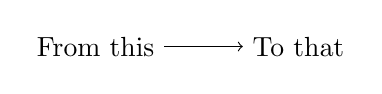
\begin{tikzpicture}
			\draw[->] (0,0) node[left] {From this} -- (1,0) node[right] {To that};
		\end{tikzpicture}
	\end{posterbox}
	\begin{posterbox}[posterblue]{This is a very boring box, but this shows that the title can be arbitrarily long and will wrap to the next line}
		Nothing to see here.
	\end{posterbox}
	\begin{posterbox}{First column last box}
		\lipsum[2]
	\end{posterbox}
\end{postercolumn}
% And here we use the remaining 0.7 of the total width.
\begin{postercolumn}[0.7]
	\begin{posterbox}[postergreen]{Second column top box}
		Test
	\end{posterbox}
	\begin{posterbox}{}
		This box has no title!
	\end{posterbox}
	\begin{posterbox}[posterpurple]{Important}
		\lipsum[3]
	\end{posterbox}
	% This is what enables advanced layouts: posterarea.
	% It allows nesting layouts inside columns.
	% The posterarea becomes the parent and any fractional 
	% measures will be with respect to the posterarea width and height.
	%
	% Syntax of posterarea:
	% \begin{posterarea}[number of columns][width][height]
	%     Columns and posterboxes can be placed here.
	% \end{posterarea}
	% Both width and height are specified as fractions of the parent area.
	\begin{posterarea}[2][][0.6]
		\begin{postercolumn}[0.4]
			% Posterspacer adds vertical space, useful for spacing elements.
			% The unit is specified as a fraction of the parent's height.
			\posterspacer{0.1}
			\begin{posterbox}[posterblue]{Nested column}
				\lipsum[4-5]
			\end{posterbox}
			\begin{posterbox}[posterorange]{}
				\begin{tikzpicture}
					\begin{axis}[
						axis y line=center,
						axis x line=middle,
						xmax=10,xmin=-1,
						ymin=-5,ymax=10,
						xlabel=$x$,ylabel=$y$,
						xtick={-10,...,10},
						ytick={-10,...,10},
						width=\textwidth,
						anchor=center,
						]
						\addplot {x^2-7*x+10};
					\end{axis}
				\end{tikzpicture}
			\end{posterbox}
			\begin{posterbox}[posteryellow]{Nested column, bottom left}
				Short text
			\end{posterbox}
		\end{postercolumn}
		\begin{postercolumn}[0.6]
			\begin{posterbox}[postergreen]{Boxbox}
				\lipsum[5]
			\end{posterbox}
			\begin{posterbox}{}
				This box has no title!
			\end{posterbox}
			% Posterspacer adds vertical space, useful for spacing elements.
			% The unit is specified as a fraction of the parent's height.
			\posterspacer{0.1}
			\begin{posterbox}[posterpurple]{Conclusions}
				\lipsum[6]
			\end{posterbox}
		\end{postercolumn}
	\end{posterarea}
	\begin{posterbox}{References}
		Thank you for reading this far...
	\end{posterbox}
\end{postercolumn}
\end{document}
